\documentclass[a4paper,titlepage]{article}

% Plantilla para documentos de la UNED creada por Martín "n3m1.sys" Romera Sobrado

% Informe de la PEC de la convocatoria de Septiembre de 2020 para la asignatura de 
% Ingeniería de Computadores 3 del grado de Ingeniería Informática de la UNED

% Para compilar hace falta el paquete pygmentize instalado en el sistema junto a todas las librerías sty utilizadas en el documento

\usepackage[utf8]{inputenc}
\usepackage[spanish]{babel}
\usepackage[T1]{fontenc}
\usepackage{mathtools}
\usepackage{lmodern}
\usepackage{amssymb}
\usepackage{graphicx}
\usepackage{subcaption}
\usepackage{xcolor}
\usepackage{float}
\usepackage{xfrac}
\usepackage{caption}
\usepackage{fancyhdr}
\usepackage{listings}
\usepackage[a4paper, total={6in, 8in}]{geometry}

\definecolor{gris}{RGB}{220,220,220}
\newcommand{\titulo}{Práctica}
\newcommand{\tituloc}{PEC}
\newcommand{\convoc}{Sep20}
\newcommand{\asig}{Ingeniería de Computadores 3}
\newcommand{\asigc}{IC3}

\pagestyle{fancy}
\fancyhf{}
\rhead{Martín Romera Sobrado}
\lhead{\asigc-\tituloc-\convoc-UNEDII}
\cfoot{\thepage}

\usepackage{minted}

\begin{document}
	
	\title{\titulo}
	\author{Martín Romera Sobrado\\
		\small{\asig} \\
		\small{Centro Asociado de la UNED en Bizkaia} \\
		\small{email: mromera95@alumno.uned.es} \\
	}
	\maketitle
	\newpage
	\section{Ejercicio 1}
		En este ejercicio desarrollaremos un circuito que sigue la siguiente tabla para las entradas \texttt{x}, \texttt{y} y \texttt{z} y las salidas 
		\texttt{F1} y \texttt{F2}:
		\begin{table}[h]
			\centering
			\begin{tabular}{|c|c|c||c|c|}
				\hline
				\texttt{x} & \texttt{y} & \texttt{z} & \texttt{F1} & \texttt{F2} \\
				\hline
				0 & 0 & 0 & 0 & 0 \\
				\hline
				0 & 0 & 1 & 0 & 1 \\
				\hline
				0 & 1 & 0 & 0 & 1 \\
				\hline
				0 & 1 & 1 & 1 & 0 \\
				\hline
				1 & 0 & 0 & 0 & 1 \\
				\hline
				1 & 0 & 1 & 1 & 0 \\
				\hline
				1 & 1 & 0 & 1 & 0 \\
				\hline
				1 & 1 & 1 & 1 & 1 \\
				\hline
			\end{tabular}
			\caption{Tabla de verdad del circuito del Ejercicio 1}
			\label{t:ej1}
		\end{table}
		\subsection{Apartado A}
			En este apartado se nos pide desarrollar la \texttt{entity} del circuito, definida por 3 entradas
			(\texttt{x}, \texttt{y} y \texttt{z}) y dos salidas (\texttt{F1} y \texttt{F2}). El código de este
			apartado es el siguiente:\\
			\inputminted[]{vhdl}{../Ejercicio1/vhdl/ej1_a.vhd}
		\subsection{Apartado B}
			En este apartado se pide desarrollar la \texttt{architecture} para la \texttt{entity} del apartado
			anterior, definiendo el comportamiento del circuito. Para ello definimos las siguientes funciones 
			booleanas:\\
			\[F1 = yz + x(y + z)\]
			\[F2 = \overline{x}(y \oplus z) + x\overline{(y \oplus z)}\]
			En lo que se traduce en el siguiente código vhdl:
			\inputminted[]{vhdl}{../Ejercicio1/vhdl/ej1_b.vhd}
		\subsection{Apartado C}
			Para este apartado tenemos que diseñar un circuito con puertas lógicas que defina las funciones lógicas
			de la tabla \ref{t:ej1}. El circuito resultante es el siguiente:\\
			\begin{figure}[h]
				\centering
				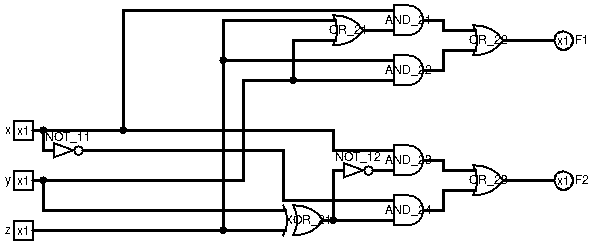
\includegraphics[width=\textwidth]{../Ejercicio1/circuitos/ejercicio1_c.png}
				\caption{Circuito para el Apartado C del Ejercicio 1}
				\label{f:circ_ej1_c}
			\end{figure}

			A partir de este circuito tenemos que definir la \texttt{entity} y \texttt{architecture} de cada una de las
			puertas lógicas del circuito en vhdl. El código es el siguiente:\\
			\inputminted[]{vhdl}{../Ejercicio1/vhdl/ej1_c.vhd}
		\subsection{Apartado D}
			Aprovechando las puertas lógicas del anterior apartado, en este las utilizaremos para definir 
			\texttt{architecture} de la estructura de la \texttt{entity} del apartado 1. Siguiendo el circuito 
			de la figura \ref{f:circ_ej1_c} obtenemos el siguiente código:\\
			\inputminted[breaklines]{vhdl}{../Ejercicio1/vhdl/ej1_d.vhd}
		\subsection{Apartado E}
			Finalmente en este apartado se nos pide comprobar el correcto funcionamiento de ambas \texttt{architecture}
			mediante un \textit{testbench}, y comprobando visualmente los cronogramas resultantes. El código del testbench es 
			el siguiente:\\
			\inputminted[breaklines]{vhdl}{../Ejercicio1/vhdl/ej1_e.vhd}

			Para compilar y simularlo, en mi caso hago uso de \textit{ghdl} junto al \textit{Makefile} que he 
			escrito para facilitarme la tarea. Para observar los cronogramas desde los archivos \textit{vcd}, 
			uso el programa \textit{GTKWave}. Los resultados son los siguientes:\\
			\begin{figure}[ht]
				\centering
				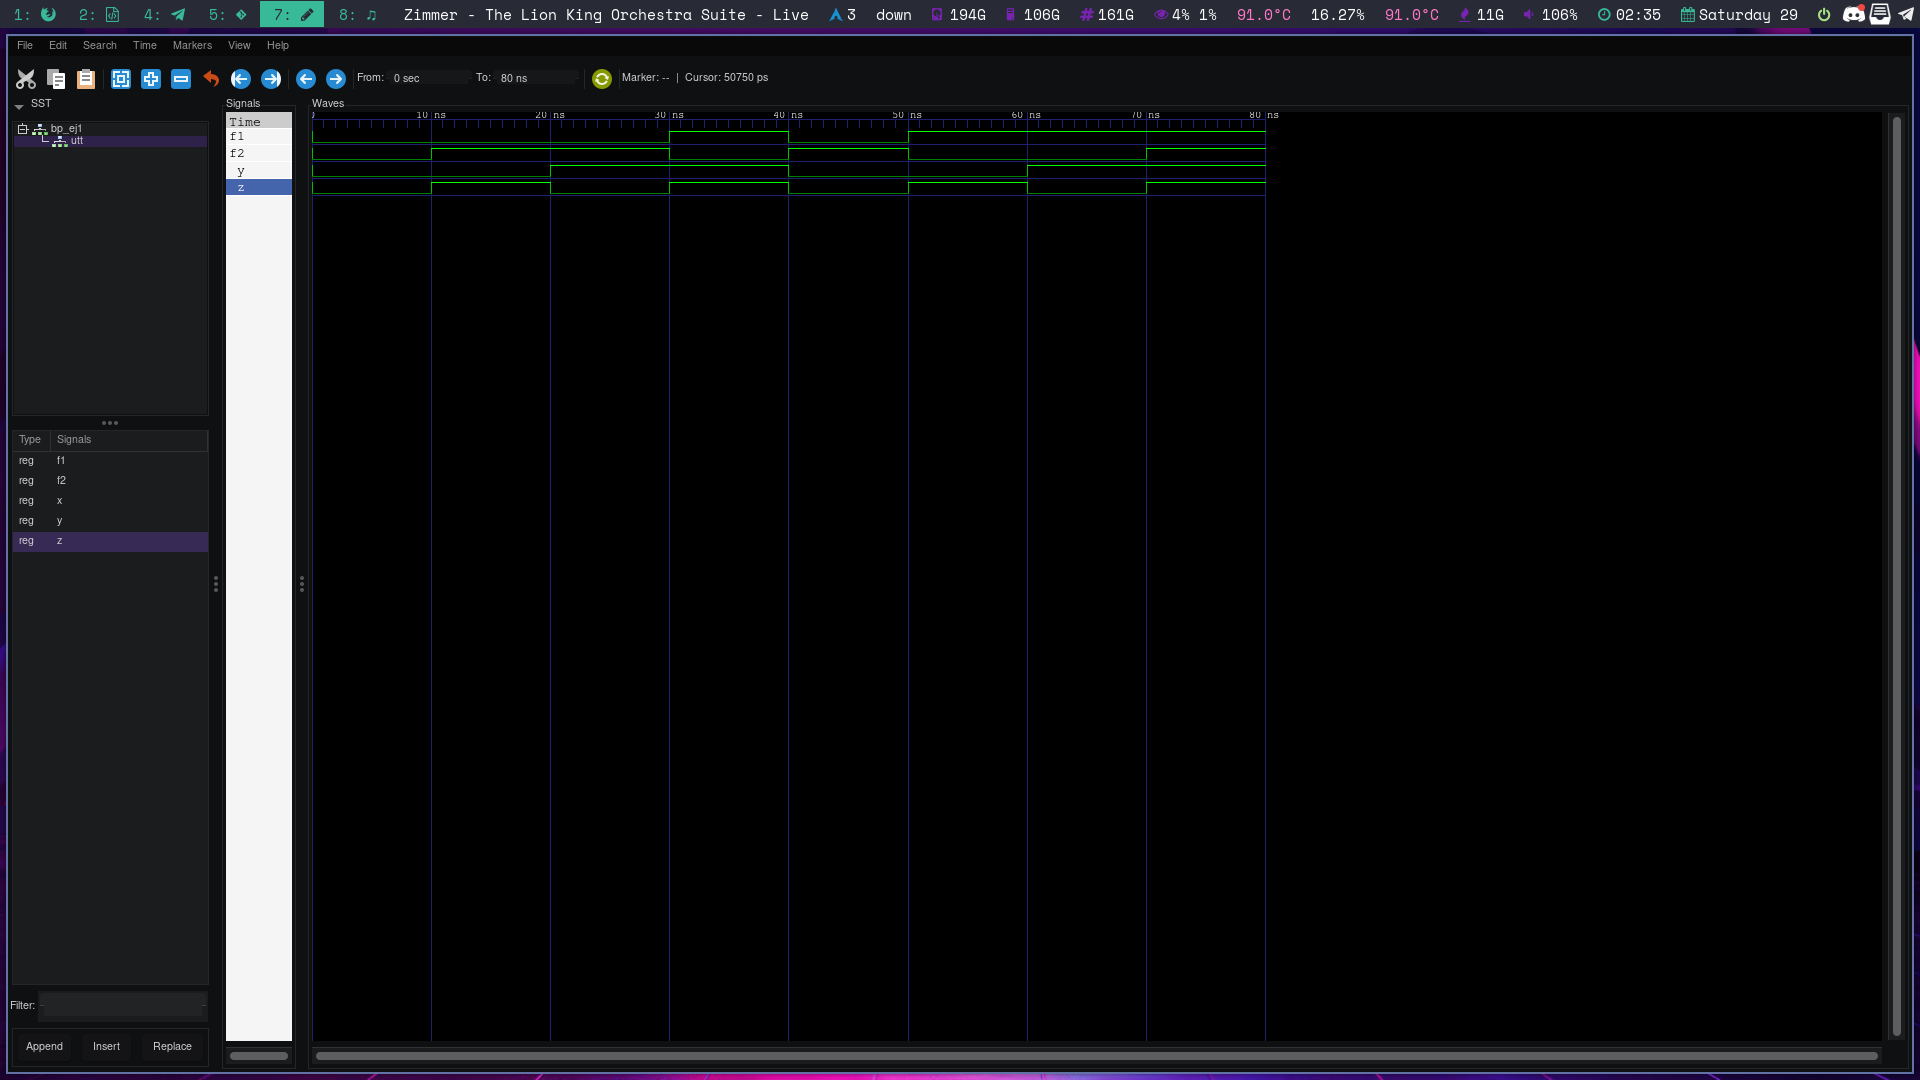
\includegraphics[width=\textwidth]{../Ejercicio1/wave/gtkwave_ej1_comportamiento.png}
				\caption{Cronograma del ejercicio 1 con la \texttt{architecture} apartado b}
				\label{f:ej1_comportamiento}
			\end{figure}
			\begin{figure}[ht]
				\centering
				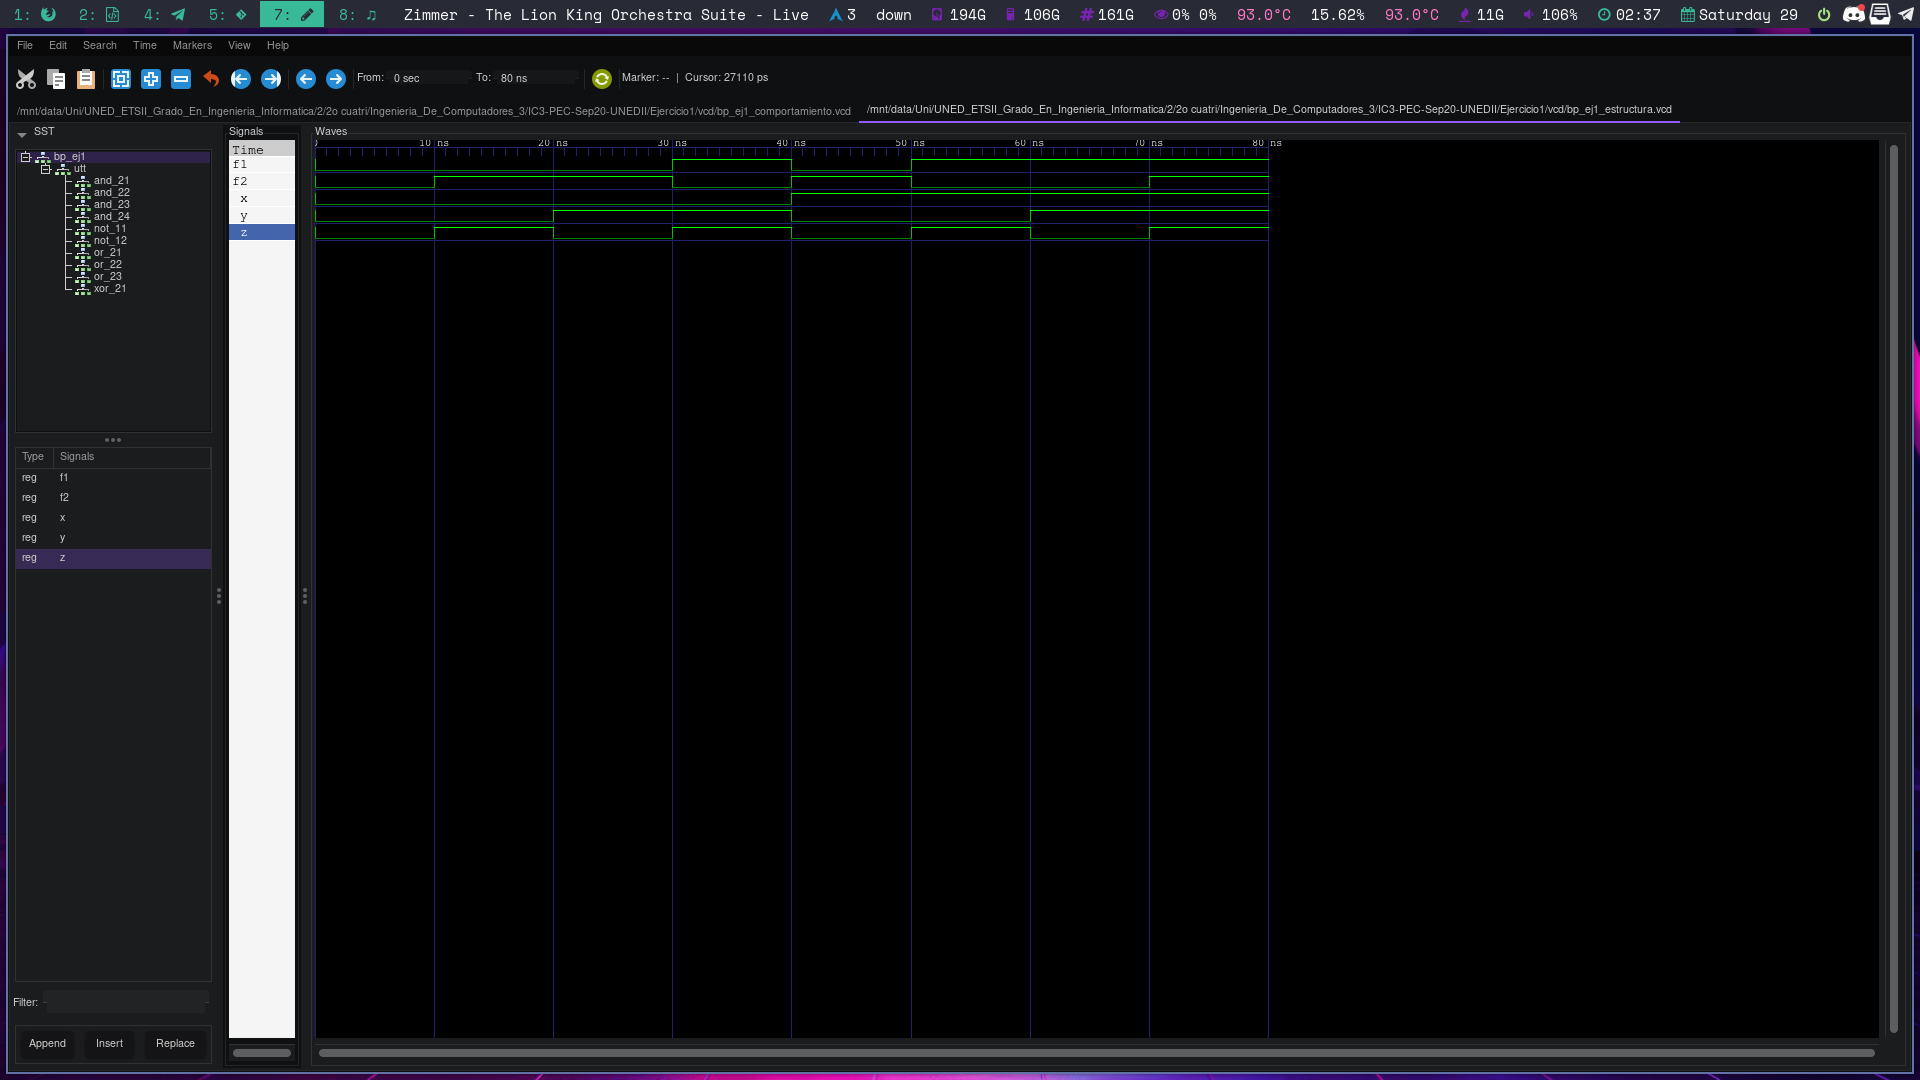
\includegraphics[width=\textwidth]{../Ejercicio1/wave/gtkwave_ej1_estructura.png}
				\caption{Cronograma del ejercicio 1 con la \texttt{architecture} apartado d}
				\label{f:ej1_estructura}
			\end{figure}

			Si comprobamos ambos cronogramas con la tabla de verdad del cuadro \ref{t:ej1} vemos que el
			circuito funciona correctamente.
		
			\newpage
		
		\section{Ejercicio 2}
			Para este ejercicio se nos propone un circuito como el siguiente:\\
			\begin{figure}[h!]
				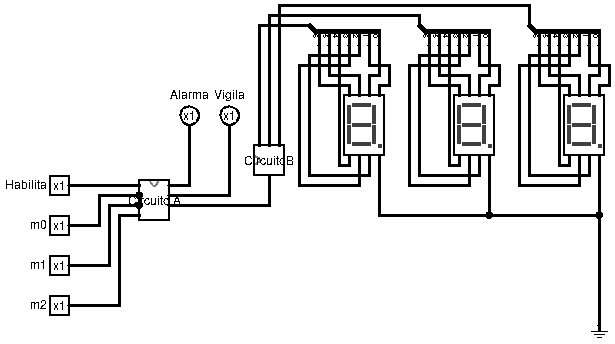
\includegraphics[width=\textwidth]{../Ejercicio2/circuitos/circuito_principal.png}
				\caption{Circuito del ejercicio 2}
				\label{f:ej2}
			\end{figure}

			Se trata de un circuito de la alarma de un museo que funciona de la siguiente manera:\\
			Las señales \texttt{m0}, \texttt{m1} y \texttt{m2} corresponde a sensores de movimiento de
			las 3 habitaciones del museo. Si ninguno detecta movimiento (todos a `0'), entonces se activará
			la señal ``vigila'', que dirá al guarda que tiene que vigilar. La señal habilita indica si la alarma
			está encendida, la cual se activa si detecta movimiento en al menos dos habitaciones. Para indicar que
			la alarma está encendida, el \texttt{Circuito A} manda la señal ``00'' al \texttt{Circuito B} el cual 
			es el responsable de de mostrar la palabra \texttt{On} en los 7 segmentos. En el caso de que la señal habilita 
			esté a `0', la alarma estará apagada haciendo que el \texttt{Circuito A} mande la señal ``00'' al
			\texttt{Circuito B} mostrando este la palabra \texttt{Off} por los 7 segmentos. Los 7 segmentos se controlan
			mediante un vector de señales lógicas de 7 bits de la siguiente manera:
			\begin{figure}[h]
				\centering
				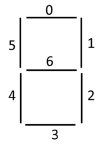
\includegraphics{img/7seg.png}
			\end{figure}
			\subsection{Apartado A}
				En este apartado tenemos que definir la estructura del \texttt{Circuito A} elabora las \texttt{entity} 
				y \texttt{architecture} de cada una de las puertas lógicas, y usando estas últimas la \texttt{entity}
				y \texttt{architecture} del circuito. El diagrama del circuito sería el siguiente:\\
				\begin{figure}[h]
					\centering
					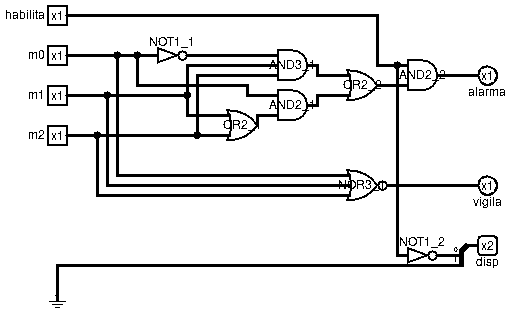
\includegraphics[width=\textwidth]{../Ejercicio2/circuitos/circuito_a.png}
					\caption{Circuito A}
					\label{f:ej2_a}
				\end{figure}

				De lo que desarrollamos el siguiente código en vhdl:
				\inputminted[breaklines]{vhdl}{../Ejercicio2/vhdl/ej2_a.vhd}
			\subsection{Apartado B}
				Para este apartado hay que definir la \texttt{entity} y \texttt{architecture} del \texttt{Circuito B}. 
				Como este tiene una forma de ``decodificador selector'', haremos uso de un proceso con sentencias 
				\texttt{case/when}:\\
				\inputminted[breaklines]{vhdl}{../Ejercicio2/vhdl/ej2_b.vhd}
			\subsection{Apartado C}
				En este apartado pondremos en conjunto ambos circuitos para formar el circuito de la figura \ref{f:ej2},
				con el siguiente código:\\
				\inputminted[breaklines]{vhdl}{../Ejercicio2/vhdl/ej2_c.vhd}
			\subsection{Apartado D}
				Finalmente, de manera similar al ejercicio anterior, desarrolaremos un \textit{testbench} para comprobar
				el correcto funcionamiento del circuito entero, solo que este deberá de comprobar los casos mediante \texttt{assert}s:\\
				\inputminted[breaklines]{vhdl}{../Ejercicio2/vhdl/ej2_d.vhd}
				El cual al ejecutar, no hace que salte ningun error, logrando además el siguiente cronograma:\\
				\begin{figure}[ht]
					\begin{center}
						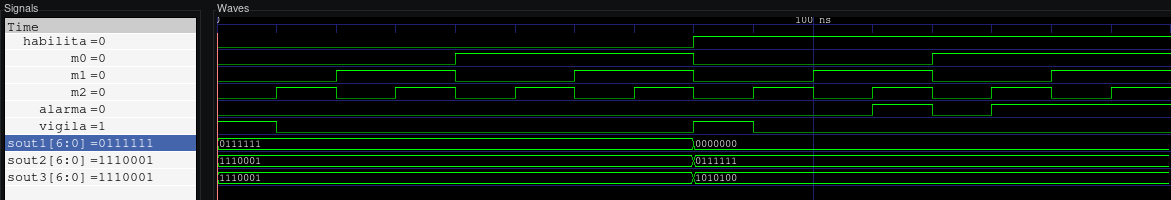
\includegraphics[width=\textwidth]{../Ejercicio2/wave/gtkwave_ej2.png}
						\caption{Cronograma del circuito completo del Ejercicio 2}
					\end{center}
					\label{f:ej2_crono}
				\end{figure}
\end{document}